\chapter{Priors, Likelihoods, and Posteriors}\label{ch:priors_posteriors}
%!TEX root = main.tex

\section{Binomial and Beta Distributions}

In Chapter~\ref{ch:parameter1} (\emph{\nameref{ch:parameter1}} on page~\pageref{ch:parameter1}) we estimated the chance, $\theta$, that a bent coin would come up heads by combining a {\em uniform prior} for $\theta$ (i.e.  all possible values are a-priori equally likely) and a {\em binomial} likelihood (i.e. given $\theta$, what is the probability of the data).  This resulted in a {\em Beta} distribution for the posterior probability for $\theta$.  

Notice what the procedure of Bayes' Recipe is and how the Bayesian inference works here.  

\be
\i Specify the prior probabilities for the models being considered
\begin{quote}
We want to estimate a quantity (which we label as $\theta$), but begin with absolutely no knowledge of its value - we have a {\em uniform} prior probability.  
\end{quote}
\i Write the top of Bayes' Rule for all models being considered
\begin{quote}
 We construct a model for how different possible values of $\theta$ influence the outcome - a model we call the {\em likelihood}.  In the case of the bent coin, the likelihood model is a {\em binomial} model, and describes the probability of flipping heads or tails given how bent the coin is (i.e. given $\theta$). 
\end{quote}
\i Put in the likelihood and prior values
\i Add these values for all models
\i Divide each of the values by this sum, $K$, to get the final probabilities
\begin{quote}
 Once we observe data, we can combine the {\rm prior} and the {\em model} or {\em likelihood} using the Bayes' recipe, and obtain the {\em posterior} distribution for the unknown value, $\theta$, giving us the probability for each value, now updated with our new observations.  
\end{quote}
\ee

The last couple of steps of the recipe, for simple cases, is done by the mathematicians so we don't have to manually add and divide as we did in the previous chapters.  In the case of the coin flips we get:

\beqn
\underbrace{{\rm Beta}(\theta|{\rm data})}_{\rm posterior\ probability} \sim \overbrace{ {\rm Binomial}({\rm data}|\theta)}^{\rm likelihood}\times \underbrace{{\rm Uniform}(\theta)}_{\rm prior\ probability}
\eeqn

From this {\em Beta} distribution, we can get the most likely values (i.e. maximum probability value) for the unknown quantity of interest, $\theta$, our {\em uncertainty} in this quantity (i.e. the {\em width} of the {\em Beta} distribution) consistent with the known data.  In other words, the posterior probability summarizes all of our knowledge about the parameter of interest given the data.


\section{The Normal Distribution - Properties}\label{sec:normaldist}

The {\em Normal} distribution, also referred to as the {\em Gaussian} distribution,\footnote{The distribution is named after  Carl Friedrich Gauss who introduced it in 1809. However, it has been called in the past the Gauss-Laplacian distribution, due the the fact that Pierre Simone de Laplace was the first to apply it to real problems, and proved a number of very useful properties of it.} is by far the most commonly occurring distribution in all of statistical inference, so it requires some special attention.

\subsection{The Shape}

The shape of the Normal distribution is sometimes described as {\em bell-shaped}, as shown in Figure~\ref{fig:bell}, and is thus referred to as the bell-curve (although there are several other mathematical functions which are bell-shaped).  The function is referred to as ${\rm Normal}(\mu,\sigma)$ where $\mu$ and $\sigma$ are parameters of the model. (see Appendix~\ref{sec:greek} on page~\pageref{sec:greek} for a review of greek letters)

\begin{figure}
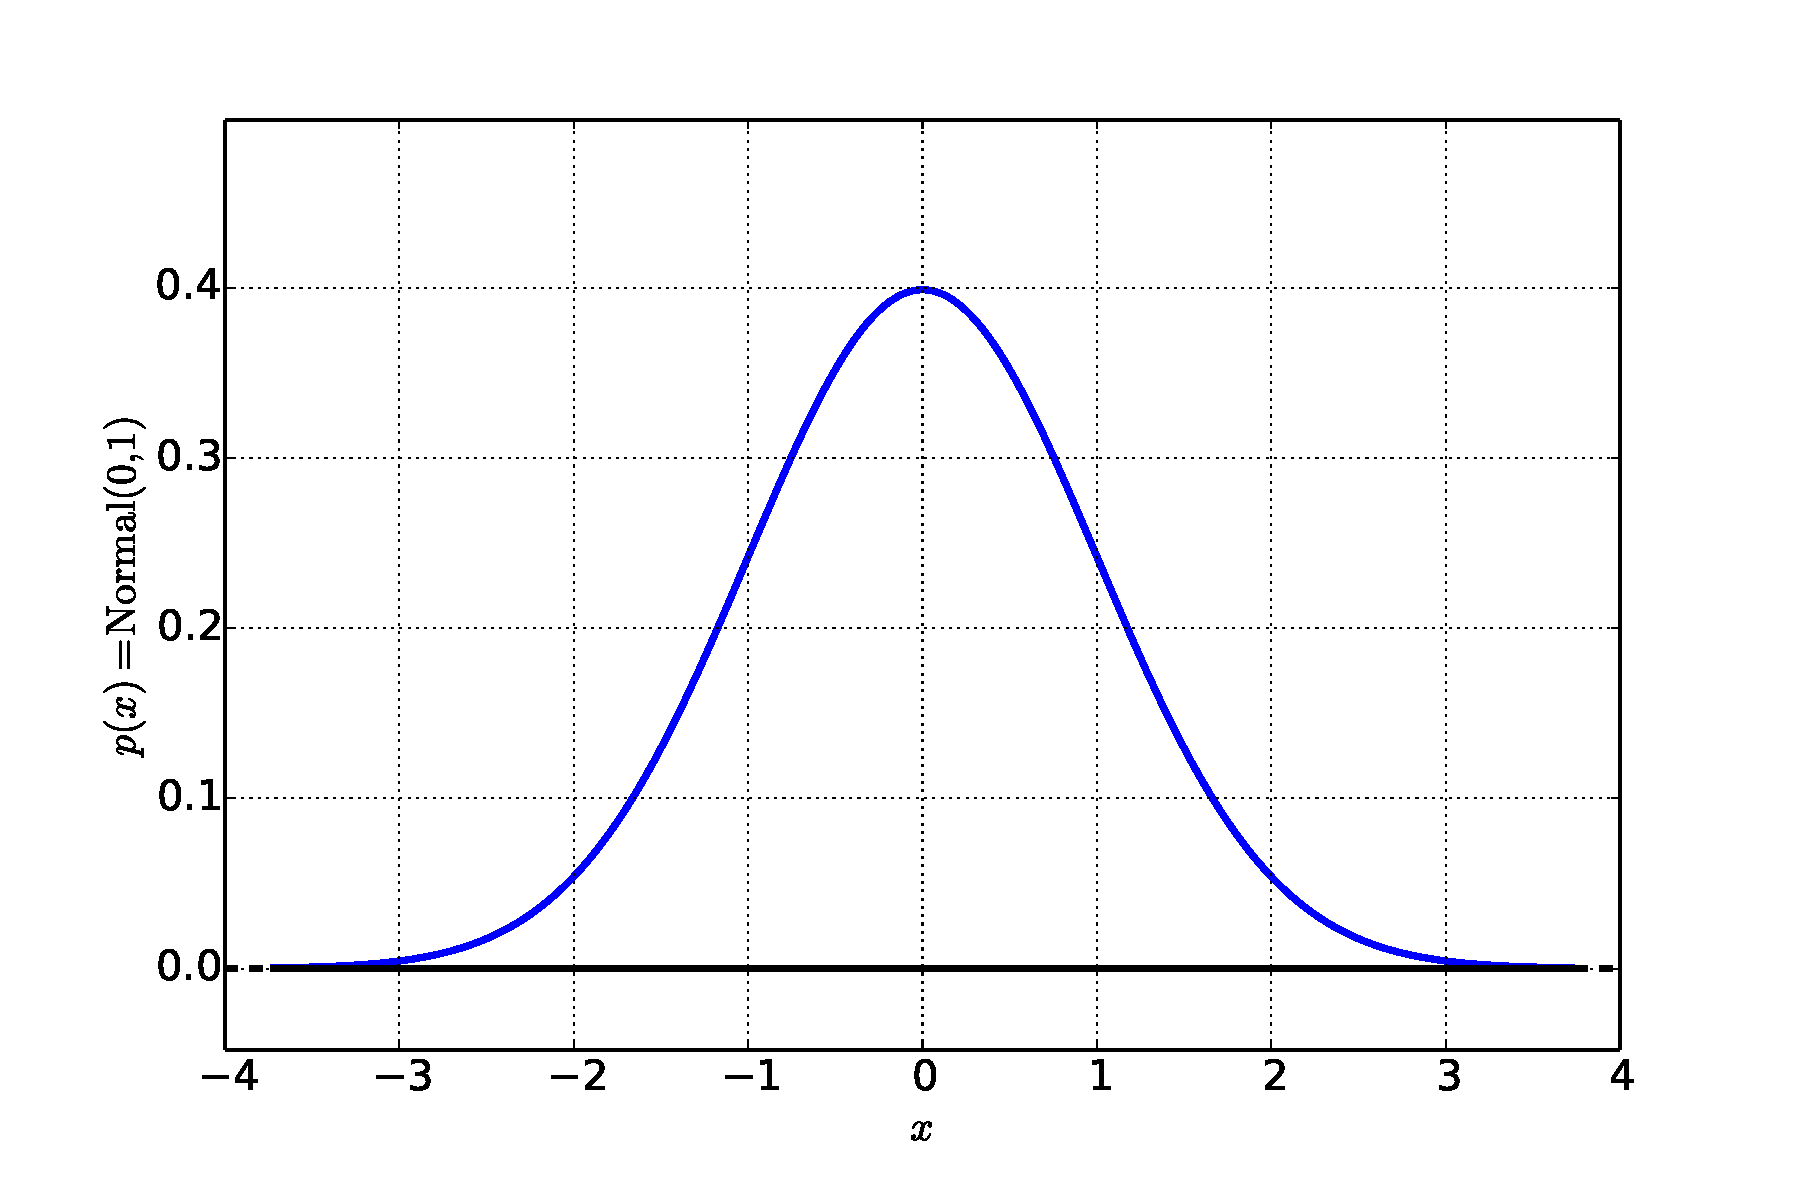
\includegraphics{gaussian1}
\caption{The Normal Distribution.}
\label{fig:bell}
\end{figure}

\subsection{The location parameter, $\mu$}

The location parameter (see Figure~\ref{fig:gaussian_mu}) is the value of $x$ for which the Normal distribution has a maximum probability.  In a real sense, it is the {\em middle} of the distribution, and the best estimate of $x$.  For the Normal distribution the location parameter, $\mu$, is at once the mean, median and mode of the distribution.

\begin{figure}
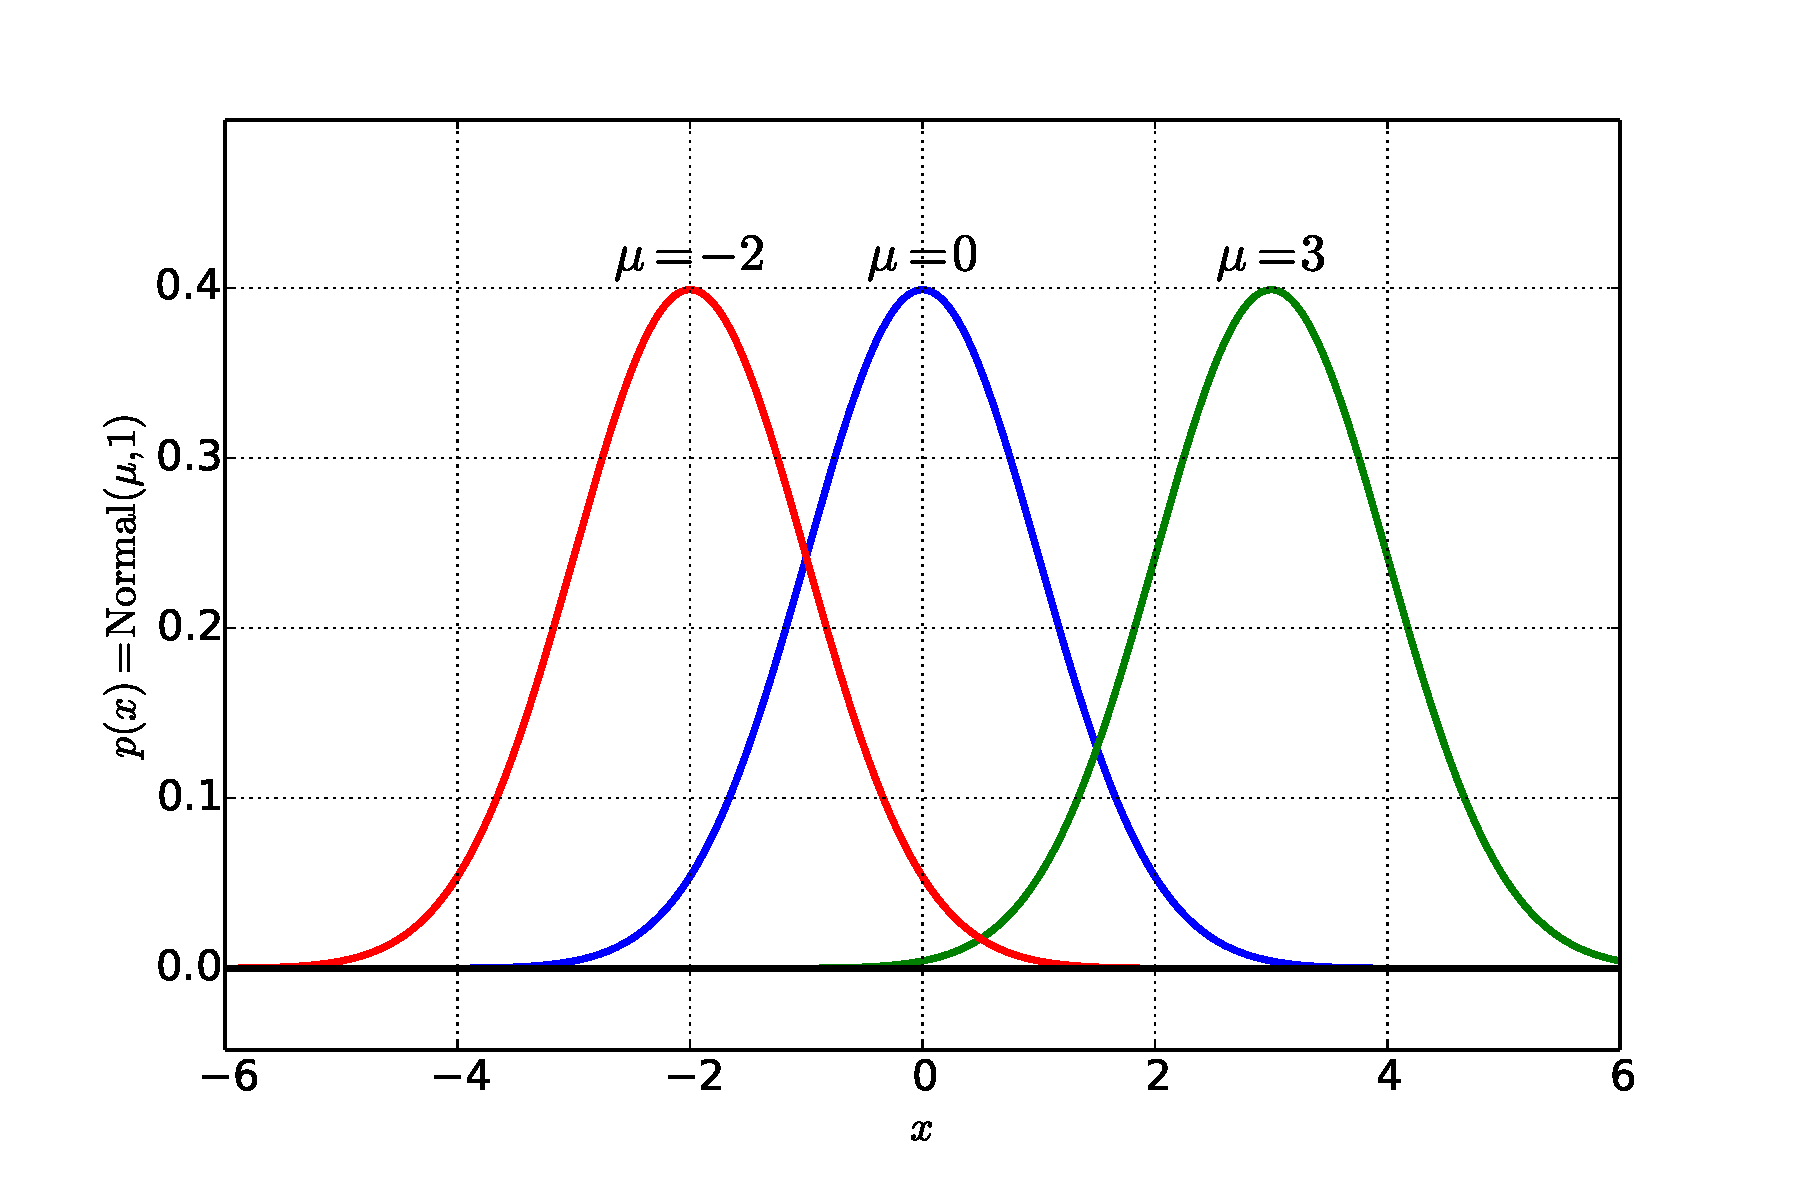
\includegraphics{gaussian_mu}
\caption{The Normal distribution with different location parameters, $\mu$.}
\label{fig:gaussian_mu}
\end{figure}

\subsection{The deviation parameter, $\sigma$}

As shown in Figure~\ref{fig:gaussian_sigma} the deviation parameter, $\sigma$, is a measure of how {\em spread out} the distribution is.  As the width increases, the height goes down to keep the area under the curve constant (at 1).  As a result, more of the probability sits at \emph{larger} values of $x$ as $\sigma$ gets \emph{larger}.

Three useful properties of $\sigma$ for the Normal distribution are the following:
\be
\i the Normal distribution value at the maximum (i.e. at $x=\mu$) is around 2.7 times larger than the value one-$\sigma$ away from the maximum (at $x=\mu-\sigma$ and $x=\mu+\sigma$)
\i the total probability between these two points is 65\%.  This is typically written, $\mu\pm\sigma$. 
\i 95\% of the distribution lies between $\mu-2\sigma$ and $\mu+2\sigma$ (see Figure~\ref{fig:gaussian_sigma})
\ee

 For example, writing $5\pm 2$ typically implies a Normal distribution with mean $\mu=5$ and deviation $\sigma=2$.  One is 65\% certain that the range of the estimated value is between 3 and 7, and 95\% certain that the range is between 1 and 9 (i.e. mean minus two deviations and mean plus two deviations). 


\begin{figure}
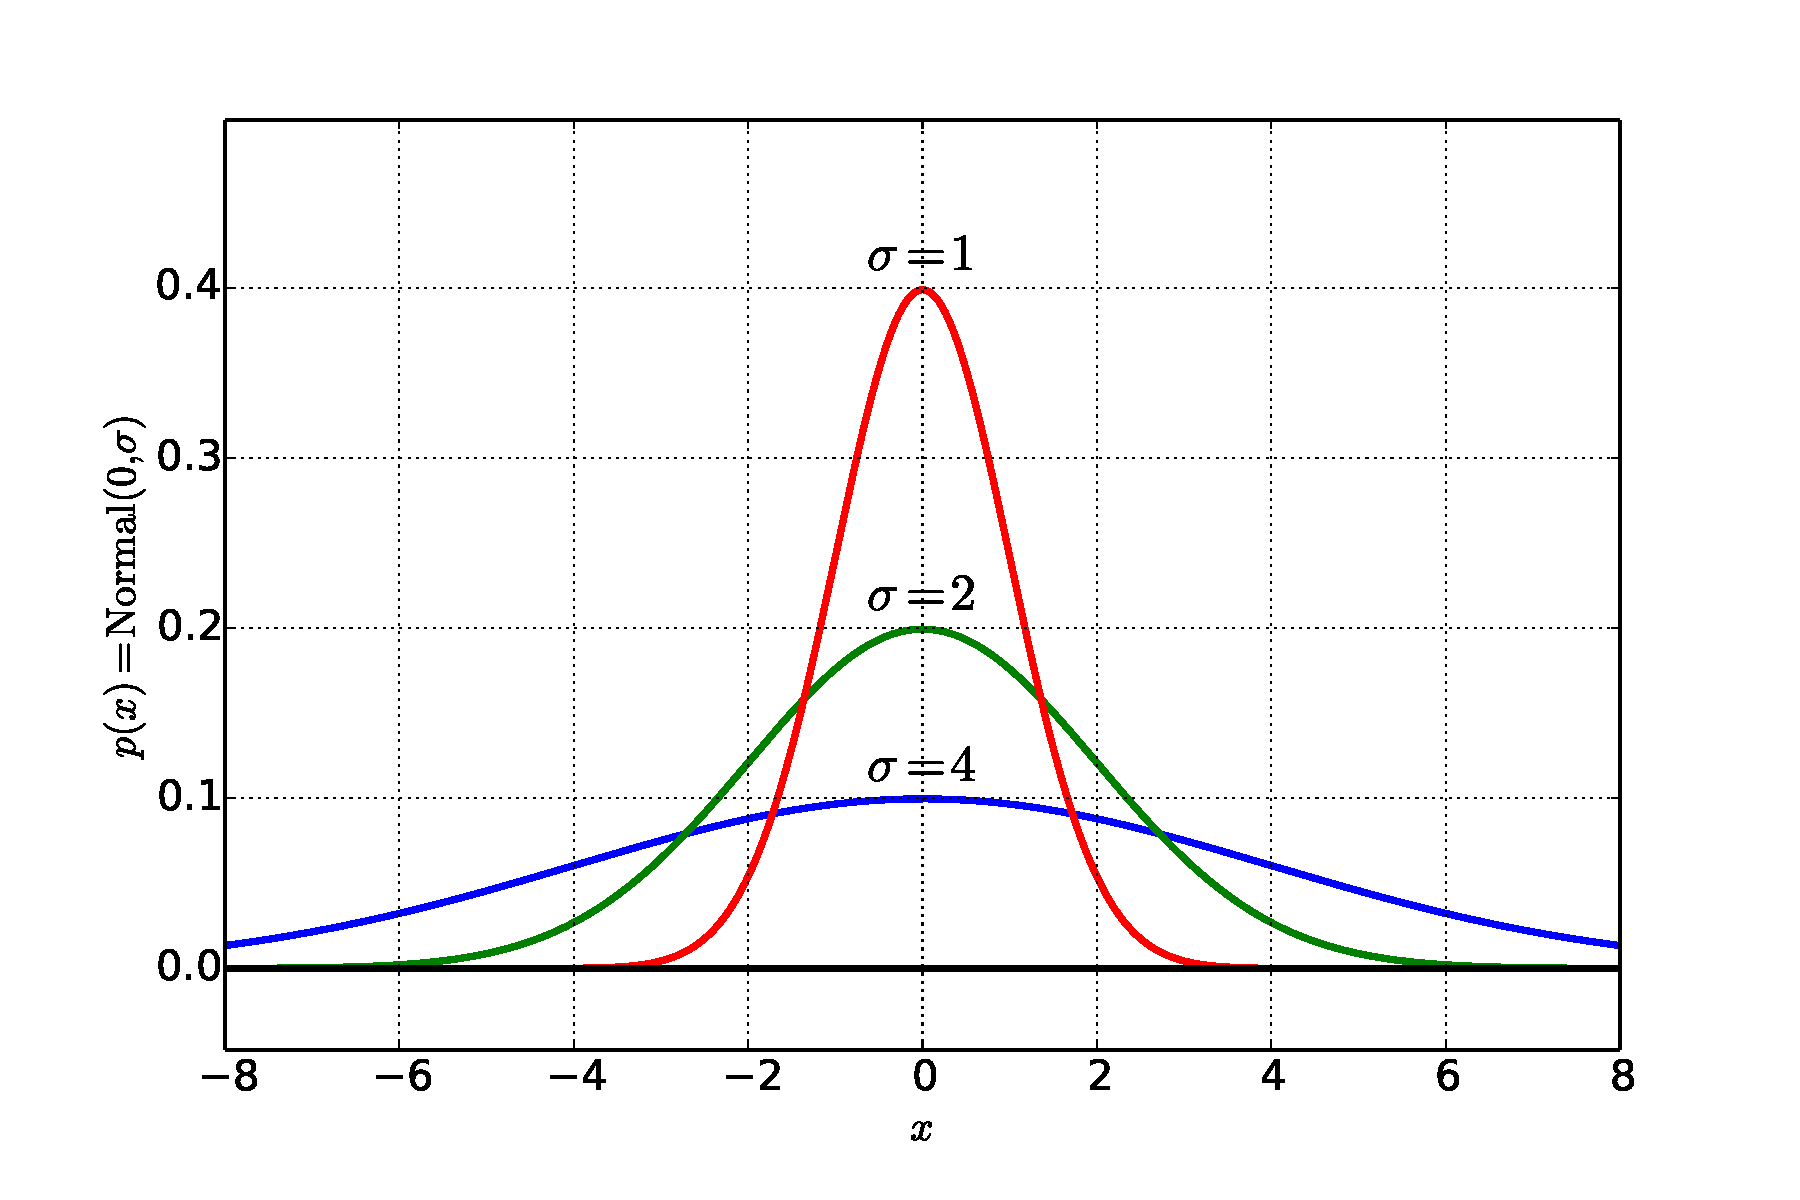
\includegraphics{gaussian_sigma}
\caption{The Normal distribution with different deviation parameters, $\sigma$.}
\label{fig:gaussian_sigma}
\end{figure}

\subsection{Summarizing the Distribution}

We can specify the Normal distribution with just the two parameters, $\mu$ and $\sigma$ - the location and deviation parameters, respectively.  However, due to its symmetry, we can summarize this distribution for all cases by looking a a single special case called the {\em standard Normal distribution}.  
\highlight{The Standard Normal Distribution}{is the Normal distribution in the special case where $\mu=0$ (the distribution is centered at $x=0$) and $\sigma=1$ (the distribution has a spread of 1).}{The Normal distribution in the special case where $\mu=0$ (the distribution is centered at $x=0$) and $\sigma=1$ (the distribution has a spread of 1).}

For any Normal distribution, the area within 1-$\sigma$ is 0.68, within 2-$\sigma$ is 0.95, and 3-$\sigma$ is 0.99.  These locations are the most prevalently used in any kind of statistical testing, and thus we will see them many times.   

\begin{figure}
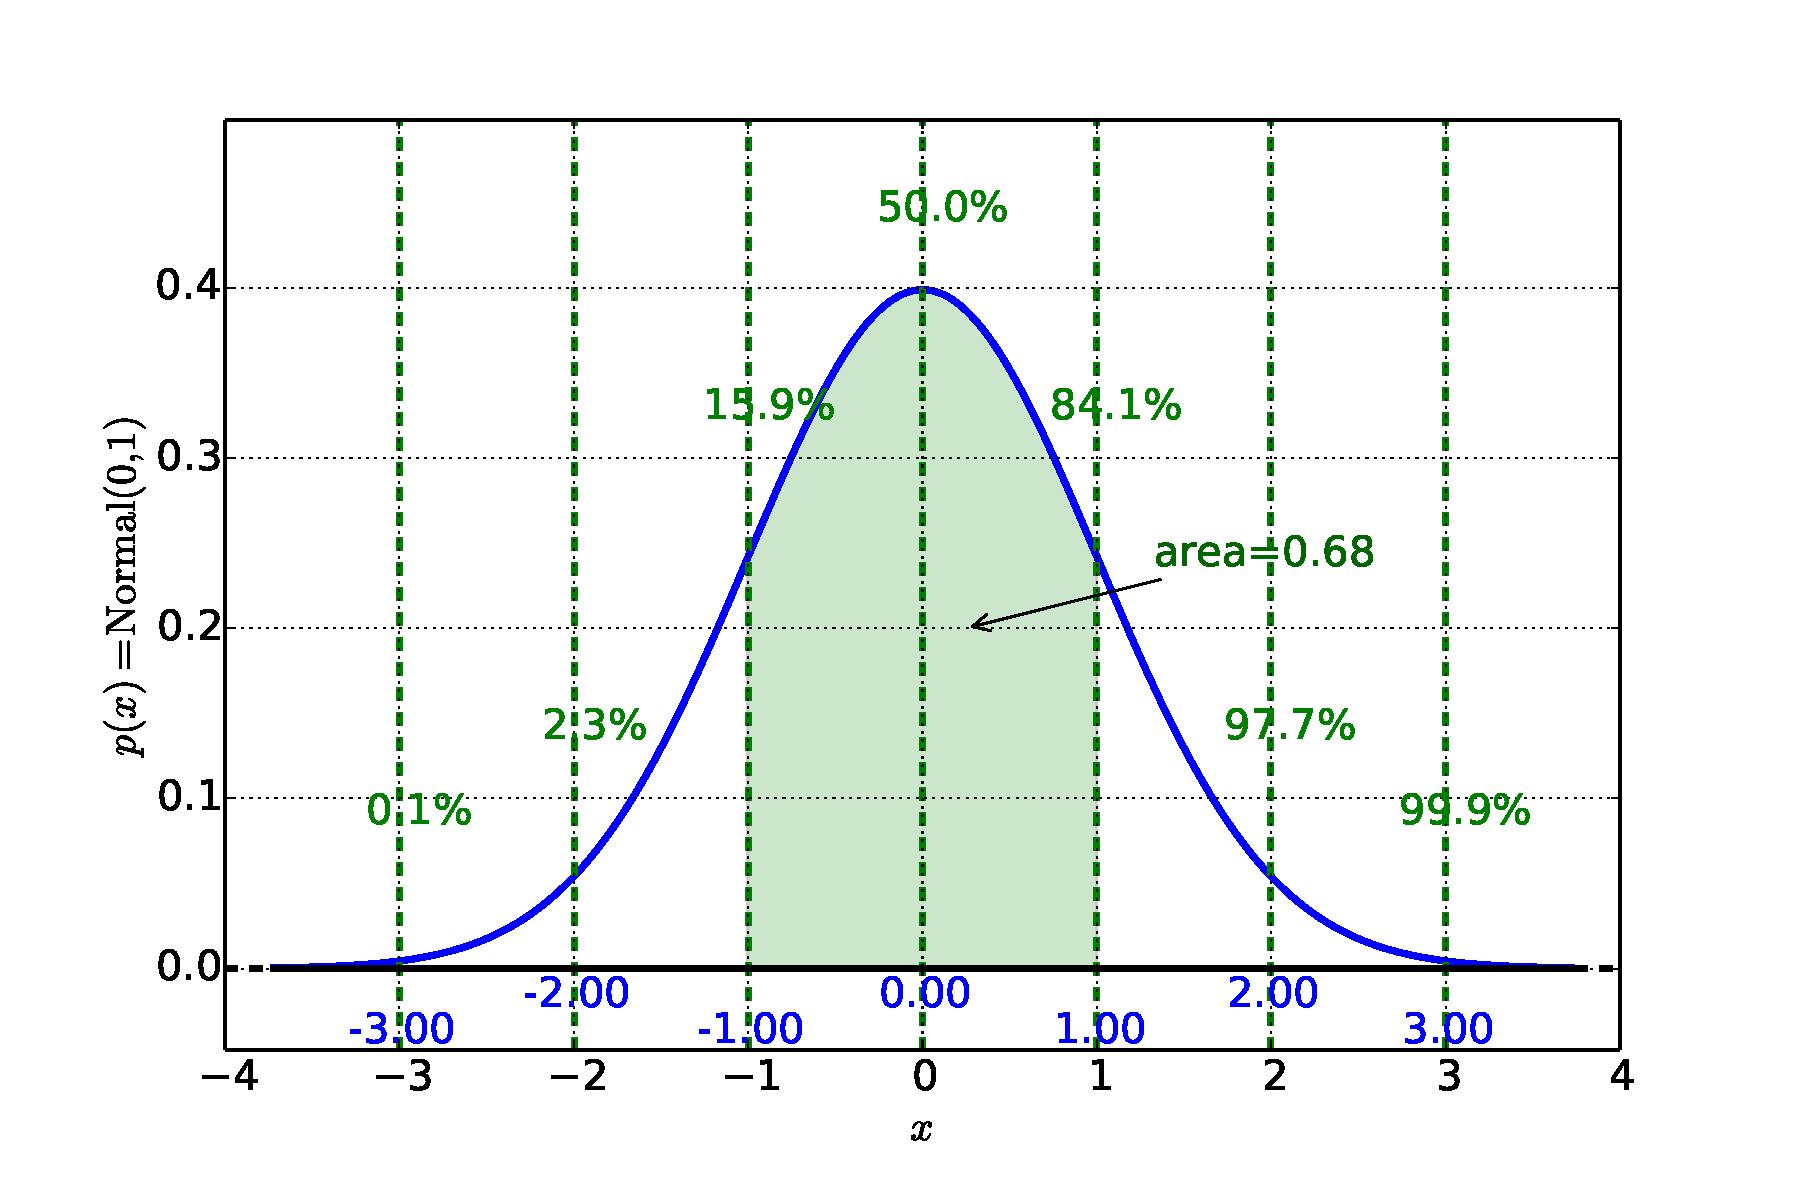
\includegraphics{gaussian_standard}
\caption{The Standard Normal Distribution (the Normal distribution in the special case where $\mu=0$  and $\sigma=1$).  The percentiles shown are for positions 1-$\sigma$ away from the center, 2-$\sigma$ away, and 3-$\sigma$ away.  The area within 1-$\sigma$ is 0.68, within 2-$\sigma$ is 0.95, and 3-$\sigma$ is 0.99.  These locations are the most prevalently used in any kind of statistical testing, and thus we will see them many times.}
\label{fig:gaussian_sigma2}
\end{figure}

\subsection{Moving from a General Normal to the Standard Normal and Back}

In order to use the table of percentiles for the standard Normal distribution, we need to be able to translate from the Normal to the standard Normal and back again.  Luckily, it is a simple process, and is one of the main reasons for using the Normal distribution - other distributions are not so easily manipulated.

To facilitate this translation, we will use the variable $x$ for the Normal distribution and $z$ for the standard Normal.  So now, we need to have a recipe for translating $x$ to $z$ (or vice versa), given $\mu$ and $\sigma$.  These recipes are:

\be
\i $x$ to $z$:  subtract $x$ by $\mu$, and divide by $\sigma$
\i $z$ to $x$:  multiply $z$ by $\sigma$ and add $\mu$
\ee

\example{Given a Normal distribution with a mean of $\mu=150$ and a $\sigma=20$, what is the most likely value?}

The most likely value is the peak of the probability distribution, $\hat{x}=\mu=150$.  

\example{Given a Normal distribution with a mean of $\mu=150$ and $\sigma=30$, what is the probability $P(x>170)$}

To use the tables in Section~\ref{sec:cumulative_normal_table} on page~\pageref{sec:cumulative_normal_table}, we first need to translate everything to the \emph{standard} Normal values.

\beqn
x=170 &\Rightarrow& z=\frac{x-150}{30} = 0.67
\eeqn

From the table in Section~\ref{sec:cumulative_normal_table} on page~\pageref{sec:cumulative_normal_table}, the area \emph{to the left} of $z=0.67$ is 0.7486.  Because we are asked the probability \emph{greater} than $x=170$ we need to have the area \emph{to the right} of the curve, or 

\beqn
P(x>170) = 1-0.7486 = 0.2514
\eeqn
or about 1/4.  In other words, with a mean $\mu=150$ and deviation $\sigma=20$, we'd expect about a quarter of the time that the value of the variable would be greater than 170.  Or, given our uncertainty of a specific value, we'd assign a probability of around 25\% to it being larger than 170.



\exercise{Normal Distribution - Probabilities}{Given a Normal distribution, with parameters $\mu=10$ and $\sigma=2$, determine the following probabilities:

\be
\i $P(x<12)$
\i $P(6<x<14)$
\i $P(2<x<12)$
\ee
}

\exercise{Normal Distribution - Likelihood}{Given a Normal distribution, with parameters $\mu=2$ and $\sigma=10$, answer the following questions (see Table~\ref{table1} on page~\pageref{table1} for reference):

\be
\i Make a qualitative plot of the distribution to help you with the other parts of the question
\i Is likely that $x>0$?
\i Above which value of $x$ is it very unlikely to observe?
\i Below which value of $x$ is it extremely unlikely to observe?
\ee
}

\exercise{Normal Distribution - Likelihood Again}{Given a Normal distribution, with parameters $\mu=2$ and $\sigma=0.5$, answer the following questions (see Table~\ref{table1} on page~\pageref{table1} for reference):

\be
\i Make a qualitative plot of the distribution to help you with the other parts of the question
\i Is likely that $x>0$?
\i Above which value of $x$ is it very unlikely to observe?
\i Below which value of $x$ is it extremely unlikely to observe?
\ee
}

\subsection{Sum and Differences}\label{sec:sumdiffnormal}

One more convenient property of the Normal distribution is that sums and differences of variables that individually have Normal distributions also have Normal distributions, although each with a different mean and deviation parameter.  The relationships are summarized as follows.  
\newpage
\highlight{Sum of two Normally distributed variables}{If we have two variables, $x$ and $y$, which have Normal distributions
\beqn
P(x) &=& {\rm Normal}(\mu_{x},\sigma_{x}) \\
P(y) &=& {\rm Normal}(\mu_{y},\sigma_{y})
\eeqn
then their sum, $x+y$, has a mean the sum of the two, $\mu_{x}+\mu_{y}$ and a deviation $\sqrt{\sigma_{x}^{2}+\sigma_{y}^{2}}$.  }{If we have two Normally distributed variables, $x$ and $y$, we have
\beqn
P(x) &=& {\rm Normal}(\mu_{x},\sigma_{x}) \\
P(y) &=& {\rm Normal}(\mu_{y},\sigma_{y}) \\
P(x+y)&=&{\rm Normal}(\mu_{x}+\mu_{y},\\
&&\sqrt{\sigma_{x}^{2}+\sigma_{y}^{2}}) 
\eeqn
}
 
One way to remember this is that the new \emph{squared} deviation parameter is the sum of the two old ones, 
\beqn
\sigma_{x+y}^{2} = \sigma_{x}^{2}+\sigma_{y}^{2}
\eeqn
 
\highlight{Differences between two Normally distributed variables}{
For differences, $x-y$, we have a new mean of $\mu_{x}-\mu_{y}$ and deviation parameter again $\sqrt{\sigma_{x}^{2}+\sigma_{y}^{2}}$. Note the ``+'' sign in the new $\sigma$, which keeps the new $\sigma$ positive which is must be by definition.
}{
\beqn
P(x-y)&=&{\rm Normal}(\mu_{x}-\mu_{y},\\
&&\sqrt{\sigma_{x}^{2}+\sigma_{y}^{2}}) 
\eeqn
(Note the ``+'' sign in the new $\sigma$.)
}

If we are asked for the distribution of a quantity with an added constant, like
\beqn
z=x+{\rm constant}
\eeqn
then the probability of $z$ is just the same as that of $x$ (i.e. Normal distribution with the same deviation), with the location parameter moved by the constant
\beqn
P(z)={\rm Normal}(\mu_{x}+{\rm constant},\sigma_{x})
\eeqn


\example{We have two Normal distributions $P(x)={\rm Normal}(\mu=8,\sigma=2)$ and $P(y)={\rm Normal}(\mu=20,\sigma=7)$.  What is the distribution for $z=y-x$? }

The distribution $P(z)$ is also a Normal distribution, with mean $\mu_{z}=20-8 = 12$ and deviation $\sigma_{z}=\sqrt{7^{2}+2^{2}}=7.3$.

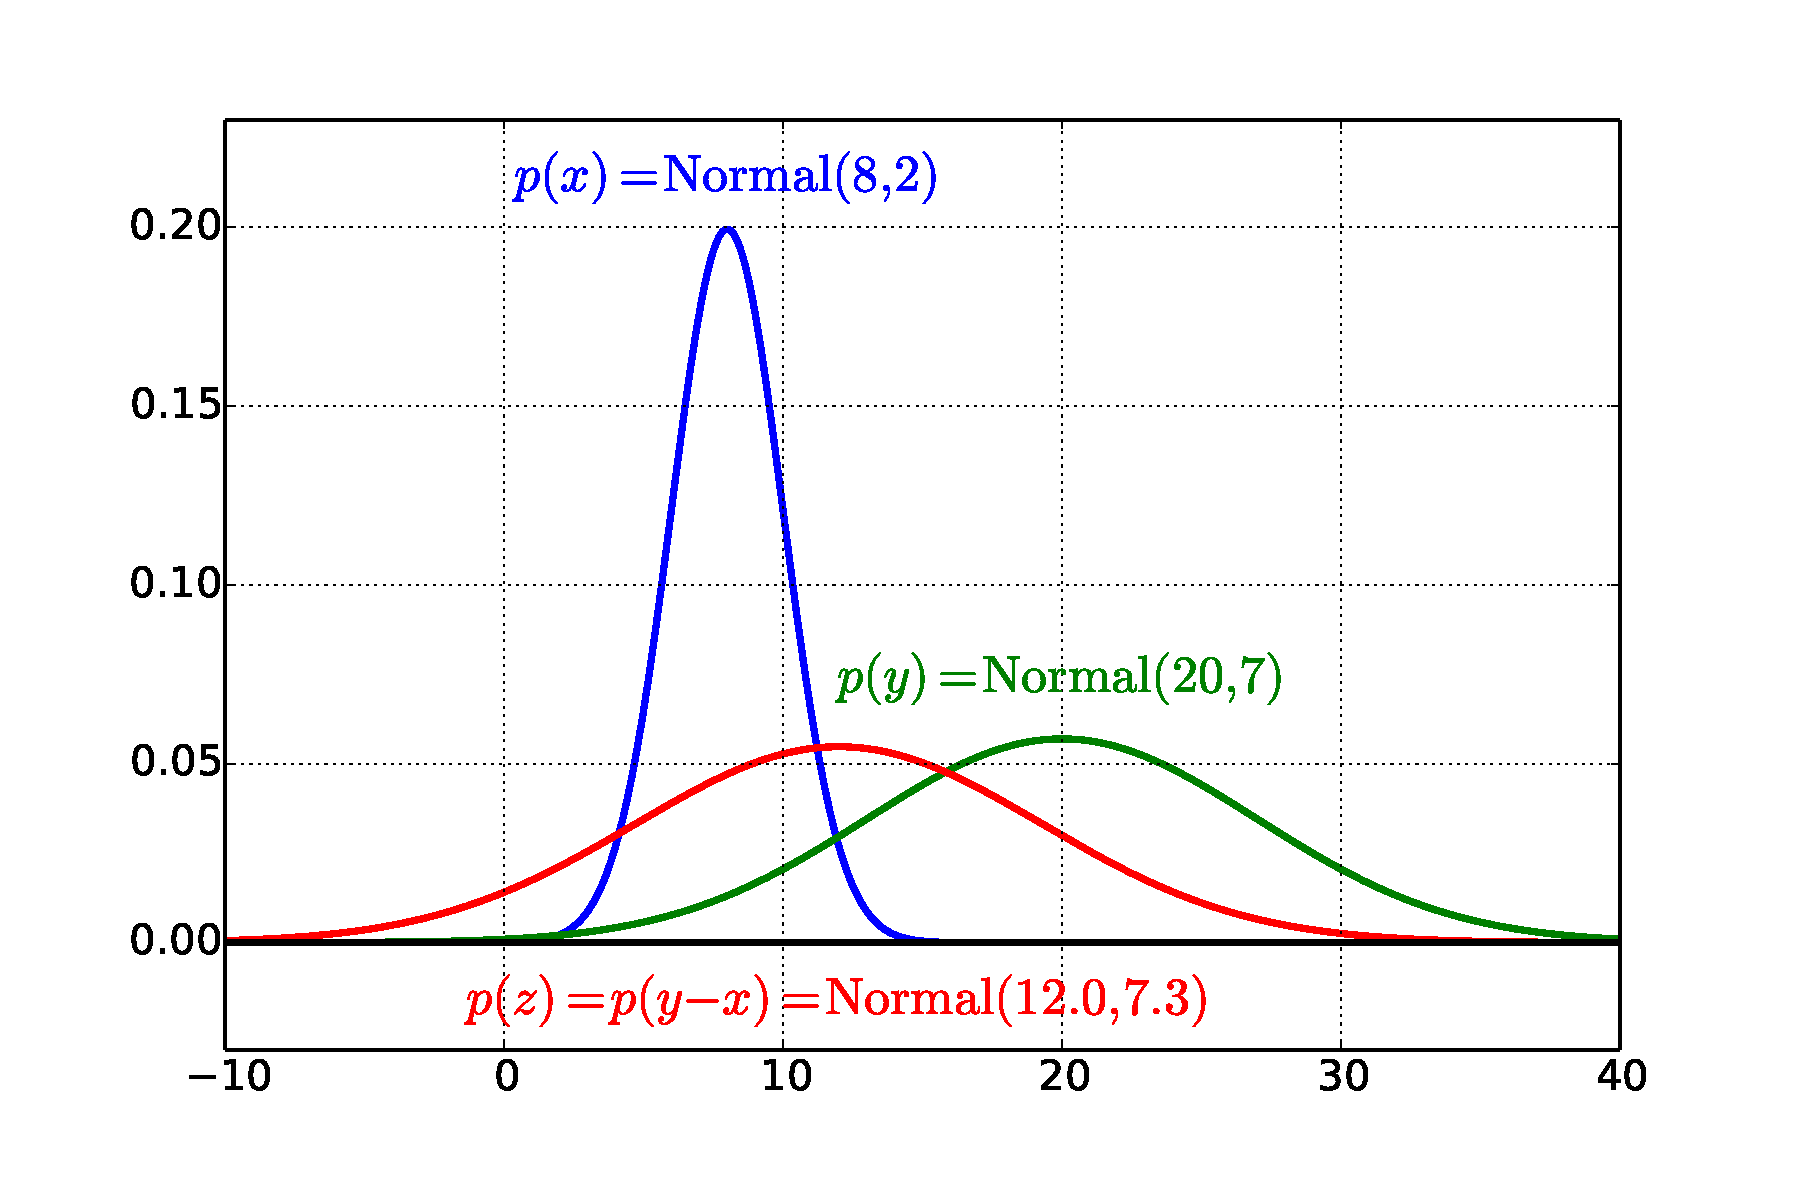
\includegraphics{gaussian_sigma_y_minus_x}


\section{The Normal Distribution - Estimating From Data}

\subsection{Estimating the mean, $\mu$, knowing the deviation, $\sigma$}\label{sec:estmean}

Typically one is provided with a series of measurements of a quantity, and we want to \emph{estimate} the value of that quantity, and have a description of our \emph{uncertainty} in the estimate.  In Chapter~\ref{ch:parameter2} (\emph{\nameref{ch:parameter2}} on page~\pageref{ch:parameter2}) we go through a number of detailed examples of this process.  Here, we simply summarize the result.  We are given:
\be
\i A series of $N$ measurements, data=$\{x_{1}, x_{2}, x_{3}, \ldots, x_{N}\}$ 
\i The real deviation, $\sigma$
\i We are modeling the data as a true value, $\mu$, with uncertainty with a likelihood from the Normal distribution with known deviation, $\sigma$, as in ${\rm Normal}(0,\sigma)$.  Further, we assume independence between the measurements.
\ee
 Since in this case we are given $\sigma$, we wish then to estimate the parameter $\mu$.  The result will be a probability distribution over $\mu$, with a best (i.e. most probable) value and an uncertainty in that value.  The result is that the distribution of $\mu$ is also a Normal distribution,\marginnote{In scientific applications, this notation is often shortened to $\mu=\bar{x} \pm \sigma/\sqrt{N}$, so it is clear what is the best estimate of $\mu$ (i.e. $\bar{x}$) and what is the uncertainty in that estimate (i.e. $\sigma/\sqrt{N}$).}
\beqn
P(\mu|{\rm data},\sigma) = {\rm Normal}(\bar{x}, \sigma/\sqrt{N})
\eeqn where the center value (and thus the most probable value of $\mu$) is given by the sample mean of the data.

\highlight{Sample Mean}{The \emph{sample mean} of a set of $N$ samples, $x_{1},x_{2},\cdots,x_{N}$ is given by
\beqn
\bar{x}\equiv\frac{x_{1} + x_{2} + x_{3} + \cdots + x_{N}}{N}
\eeqn
}{The \emph{sample mean} of a set of $N$ samples, $x_{1},x_{2},\cdots,x_{N}$ is given by
\beqn
\bar{x}\equiv\frac{x_{1} + x_{2} + x_{3} + \cdots + x_{N}}{N}
\eeqn
}

The uncertainty in $\mu$ is given by $\sigma/\sqrt{N}$.  As a consequence, larger $N$ (i.e. more data points), makes us more confident in the particular estimate for $\mu$.

\highlight{Estimate of location parameter $\mu$ given $N$ samples and $\sigma$, the known deviation}{In summary, the best estimate for the location parameter $\mu$ in the Normal distribution given a set of $N$ samples, $x_{1},x_{2},\cdots,x_{N}$ is given by
\beqn
\hat{\mu} = \frac{x_{1} + x_{2} + x_{3} + \cdots + x_{N}}{N} \pm \sigma/\sqrt{N}
\eeqn
}{The best estimate for the location parameter $\mu$ in the Normal distribution given a set of $N$ samples, $x_{1},x_{2},\cdots,x_{N}$ is given by
\beqn
\hat{\mu} = \frac{x_{1} + x_{2} + \cdots + x_{N}}{N}  \pm \sigma/\sqrt{N}
\eeqn
}


\example{Estimating the True Length of an Object}
\newcommand{\cm}{[\rm cm]}
Say we have an object, and 5 measurements of its length from the same ruler but from different people,
\begin{center}
5.1\cm, 4.9\cm, 4.7\cm, 4.9\cm, 5.0\cm
\end{center}
Say that we further know that the uncertainty (given this ruler) of one measurement has $\sigma=0.5 \cm$.\marginnote{In real measurements, there is always the problem of bias or \emph{systematic} uncertainties, where the uncertainty does not follow a Normal distribution.  We will not consider this issue here.}  What is the best estimate of the length?  The best estimate should be given by the sample mean of these 5 samples,
\beqn
\hat{\mu} &=& \frac{x_{1} + x_{2} + \cdots + x_{N}}{N} \\
 &=& \frac{5.1\cm+ 4.9\cm+ 4.7\cm+ 4.9\cm+ 5.0\cm}{5} =4.92\cm
\eeqn
with uncertainty related to the known uncertainty of a single measurement, 
\beqn
\hat{\sigma} &=& \frac{\sigma}{\sqrt{N}} \\
&=& \frac{0.5\cm}{\sqrt{5}} = 0.223\cm
\eeqn
yielding a final best estimate of

\beqn
\hat{\mu} &=& 4.92\cm\pm 0.223\cm
\eeqn
or (with $2\sigma$ range),\marginnote{The 95\% credible interval (CI) is really at the $1.96\sigma$ level, yielding $[4.481\cm,5.358\cm]$.  We will almost always approximate it as $2\sigma$ by hand, but the computer will generate the true 95\% credible interval when requested.}
\beqn
\hat{\mu} &=& 4.92\cm, 95\%\mbox{ CI} = [4.474\cm,5.366\cm]
\eeqn

\subsection{Estimating the mean, $\mu$, \emph{not} knowing the deviation, $\sigma$}\label{sec:meansigmaest}

If we are not so fortunate to be given the deviation, as in the previous case, then this parameter too must be estimated from the data.  As a first step we can estimate the deviation with the \emph{sample} deviation.

\highlight{Sample Deviation}{The sample deviation of a set of $N$ samples, $x_{1},x_{2},\cdots,x_{N}$ is given by
\beqn
S\equiv \sqrt{\frac{1}{N-1}\left( (x_{1}-\bar{x})^{2}+(x_{2}-\bar{x})^{2}+\cdots+(x_{N}-\bar{x})^{2}\right)}
\eeqn
}{The sample deviation of a set of $N$ samples, $x_{1},x_{2},\cdots,x_{N}$ is given by
\beqn
S\equiv \sqrt{\frac{1}{N-1}\left( (x_{1}-\bar{x})^{2}+\cdots+(x_{N}-\bar{x})^{2}\right)}
\eeqn
}

\highlight{Approximate estimate of location parameter $\mu$ and deviation $\sigma$ given $N$ samples}{
The posterior probability for $\mu$ and $\sigma$ given a set of $N$ samples, $x_{1},x_{2},\cdots,x_{N}$ can be approximated with
\beqn
P(\mu|{\rm data}) &\sim& {\rm Normal}(\bar{x}, S/\sqrt{N}) \\
P(\sigma|{\rm data}) &\sim& {\rm Normal}\left(S, S^{2}/\sqrt{(N-1)/3}\right)
\eeqn 
which works well if we have many ($N>30$) data points.
}{The posterior probability for $\mu$ and $\sigma$ given a set of $N$ samples, $x_{1},x_{2},\cdots,x_{N}$ can be approximated with
\beqn
P(\mu|{\rm data}) &\sim& {\rm Normal}(\bar{x}, S/\sqrt{N}) \\
P(\sigma|{\rm data}) &\sim& {\rm Normal}\left(S, \right.\\
&&\left.S^{2}/\sqrt{(N-1)/3}\right)
\eeqn 
which works well if we have many ($N>30$) data points.
}

With a smaller data set, the value of $S$ as an estimate for the deviation becomes too small.  When the estimate for $\sigma$ is too small, then the result is claiming \emph{more confidence} in the estimate of the mean, $\mu$, than is warranted.\marginnote{Because the uncertainty in the mean depends explicitly on the number of data points, it goes beyond the level of this chapter to give a form for the posterior probability distribution for the deviation, $\sigma$. }  This discrepancy depends on the number of data points, and thus it makes sense that the proper distribution should depend on the number of data points, in addition to the sample mean and deviation.  The proper, although less convenient, result is that the posterior probability for $\mu$ takes the form of the Student's $t$ distribution,
  
\highlight{Estimate of location parameter $\mu$ given $N$ samples and \emph{unknown} $\sigma$}{The posterior probability for $\mu$ takes the form of the Student's $t$ distribution,
\beqn
P(\mu|{\rm data}) = {\rm Student}_{{\rm dof}=N-1}(\bar{x}, S/\sqrt{N})
\eeqn 
This distribution requires \emph{three} numbers to specify, referred to as the mean ($\mu$), deviation ($\sigma$) and the \emph{degrees of freedom} (dof).  The degrees of freedom is defined in this case to be the number of data points less one, $N-1$.}{The posterior probability for $\mu$ takes the form of the Student's $t$ distribution,
\beqn
P(\mu|{\rm data}) = {\rm Student}_{{\rm dof}=N-1}(\bar{x}, S/\sqrt{N})
\eeqn 
This distribution requires \emph{three} numbers to specify, referred to as the mean ($\mu$), deviation ($\sigma$) and the \emph{degrees of freedom} (dof).  The degrees of freedom is defined in this case to be the number of data points less one, $N-1$.}

 
\example{Estimating the True Length of an Object...Again\label{ex:length_tdist}}
Say we have an object, and 5 measurements of its length from the same ruler but from different people,
\begin{center}
5.1\cm, 4.9\cm, 4.7\cm, 4.9\cm, 5.0\cm
\end{center}
Unlike earlier, let's say that we don't know the uncertainty (given this ruler) of one measurement What is the best estimate of the length?  Again, the best estimate should be given by the sample mean of these 5 samples,
\beqn
\hat{\mu} &=& \frac{x_{1} + x_{2} + \cdots + x_{N}}{N} \\
 &=& \frac{5.1\cm+ 4.9\cm+ 4.7\cm+ 4.9\cm+ 5.0\cm}{5} =4.92\cm
\eeqn
with uncertainty related to the sample deviation
\beqn
S^{2}&=&\frac{1}{N-1}\left( (x_{1}-\bar{x})^{2}+\cdots+(x_{N}-\bar{x})^{2}\right) \\
&=&\frac{1}{5-1}\left( (5.1\cm-4.92\cm)^{2}+(4.9\cm-4.92\cm)^{2}+(4.7\cm-4.92\cm)^{2}+\right.\\
&&\left.(4.9\cm-4.92\cm)^{2}+(5.0\cm-4.92\cm)^{2}\right) \\
&=&0.024 \cm^{2}\\
S&=&\sqrt{0.024 \cm^{2}}=0.155\cm \\
\frac{S}{\sqrt{N}}&=&\frac{0.155\cm}{\sqrt{5}}=0.069\cm
\eeqn

Looking at Table~\ref{sec:tdist_table}on page~\pageref{sec:tdist_table} with ``Degrees of Freedom'' equal to 4, we find that the 95\% credible interval for $\mu$ (between areas 0.025 and 0.975) falls $\pm 2.776 \cdot S/\sqrt{N}$, thus we have

\beqn
\hat{\mu} &=& 4.92\cm, 95\%\mbox{ CI}=[4.92\cm-2.776 \cdot 0.069\cm,4.92\cm+2.776 \cdot 0.069\cm] \\
&=&4.92\cm, 95\%\mbox{ CI}=[4.73\cm,5.11\cm]
\eeqn

Although much of this is easier with the computer, it is instructive to go through simple examples by hand.


\section{Normal Approximation}

The Normal distribution is useful for many reasons:  its simple shape, the fact that there are only two parameters which describe it, and the ease with which one can compare the general Normal distribution to the single standard Normal.  Further, it can be used as an approximation for several other distributions, under certain limits.  

\subsection{The Beta Distribution}\label{sec:beta}

We first saw the beta distribution as the posterior description in a bent-coin parameter estimation problem (see Section~\ref{sec:continuous} on page~\pageref{sec:continuous} in Chapter~\ref{ch:parameter1} (\emph{\nameref{ch:parameter1}})). The Normal approximation occurs when the number of flips gets large, compared to how likely the coin flips heads.  For notation, we will write the frequency of heads as
\beqn
f\equiv \frac{h}{N}
\eeqn

\highlight{Normal Approximation to the Beta Distribution}{
The Normal Approximation to the Beta Distribution , for large number of flips ($N$) of which a fraction $f\equiv h/N$ are successful is given by
\beqn
{\rm Beta}(h,N) \sim {\rm Normal}\left(\mu=f, \sigma=\sqrt{f(1-f)/N}\right)
\eeqn
}{The Normal Approximation to the Beta Distribution , for large number of flips ($N$) of which a fraction $f\equiv h/N$ are successful is given by
\beqn
{\rm Beta}(h,N) &\sim& {\rm Normal}\left(\mu=f, \right.\\
&&\left.\sigma=\sqrt{f(1-f)/N}\right)
\eeqn
}
To see how close this approximation can be, observe the following two cases:

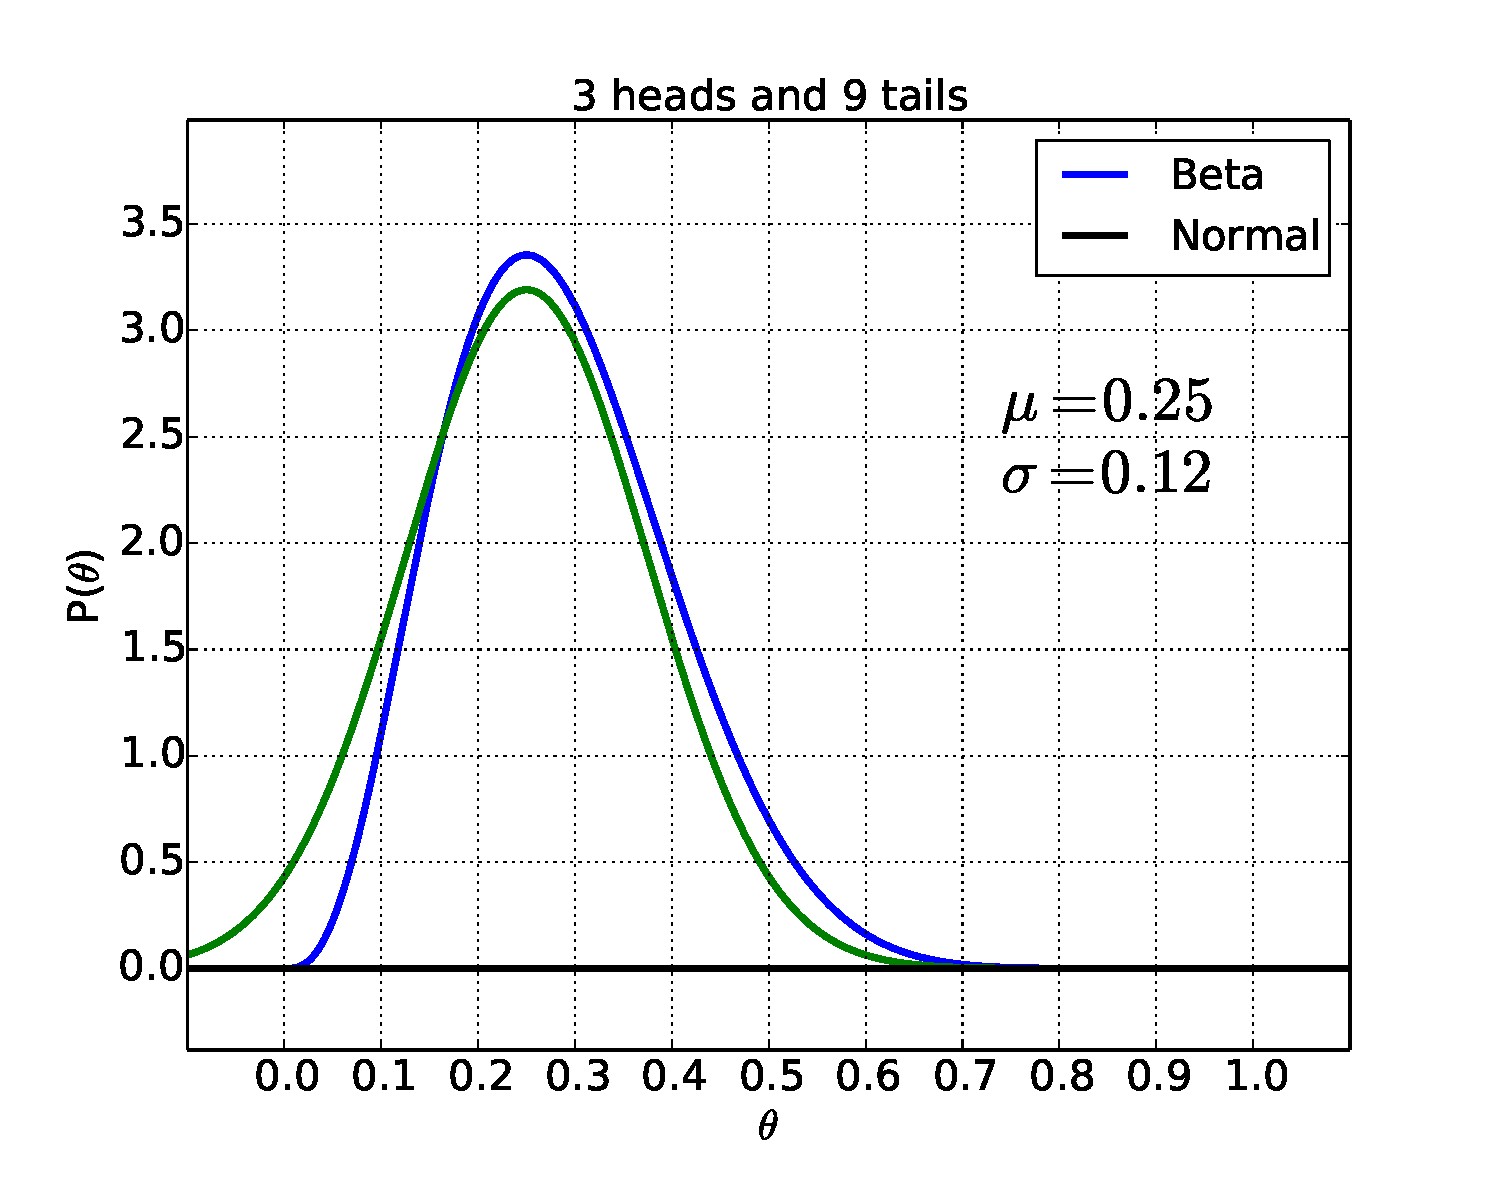
\includegraphics{beta_normal_3_12.pdf}
 
With ten times as many flips, we have

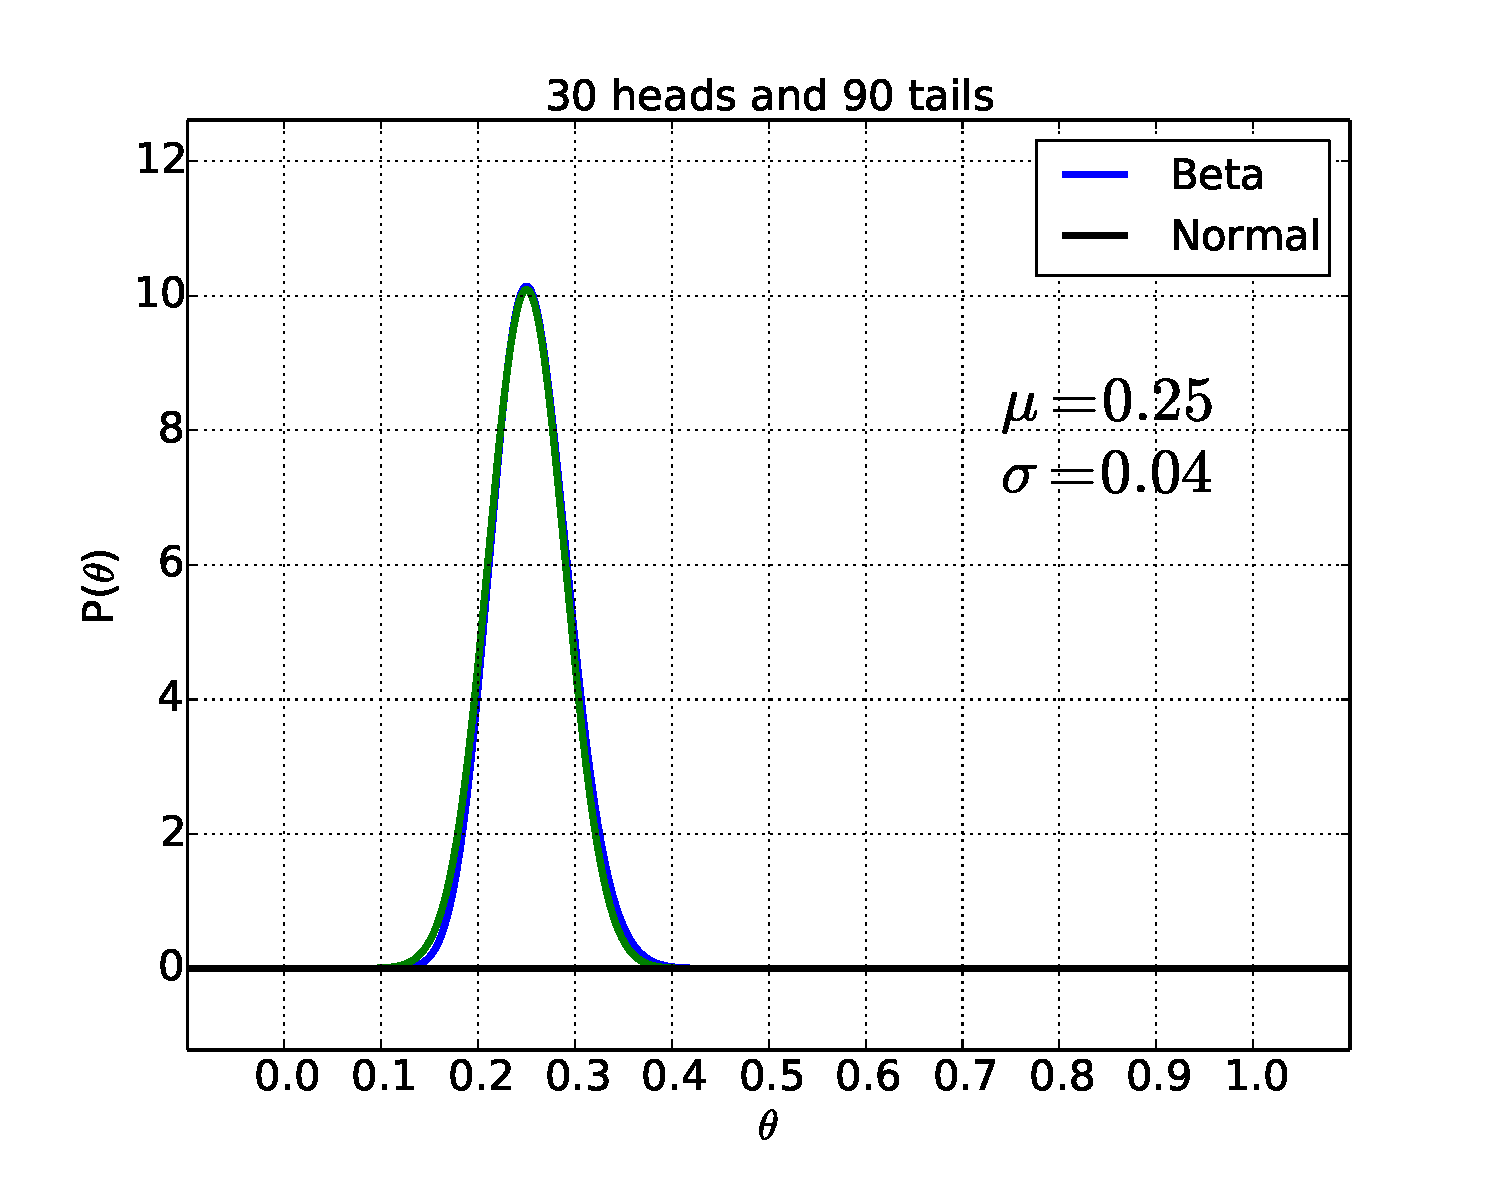
\includegraphics{beta_normal_30_120.pdf}

and the curves are so close as to be nearly identical!\marginnote{This is an {\em approximation}, and as such will certainly give seriously incorrect answers under certain circumstances.  For example, in this case, the Normal approximation predicts that there is around a 1.8\% chance that the bent coin might have a \emph{negative} $\theta$, or probability of flipping heads (look a the Normal curve to the left of $\theta=0$)!  The beta distribution is zero for any value below zero or over one, and thus will never lead to such absurd answers.  }  There still is a (small) probability for getting a negative $\theta$, which is problematic in theory but not typically in practice.  To use the properties of the Normal distribution here to quantify our uncertainty about the bent coin.  Given 30 heads and 90 tails, the best estimate for $\theta$ (i.e. the top of the curve) is 0.25.  Our uncertainty is quantified by the width of the distribution, given by $\sigma$.  Thus, we can be confident to a 95\% degree for $\theta$ within $2\sigma$, or between 0.17 and 0.33 ($0.25-2\cdot 0.04$ and $0.25+2\cdot 0.04$, respectively).


\subsection{The Binomial Distribution}

Similarly, with the (discrete) binomial distribution (see Equation~\ref{eq:binomial}) we have the Normal approximation.

\highlight{Normal Approximation to the Discrete Binomial Distribution}{
\beqn
{\rm Binomial}(N,p) = {\rm Normal}(\mu=N\cdot p,\sigma=\sqrt{N\cdot p(1-p)})
\eeqn
}{
\beqn
{\rm Binomial}(N,p) &=& {\rm Normal}(\mu=N\cdot p,\\
&&\sigma=\sqrt{N\cdot p(1-p)})
\eeqn
}

with examples

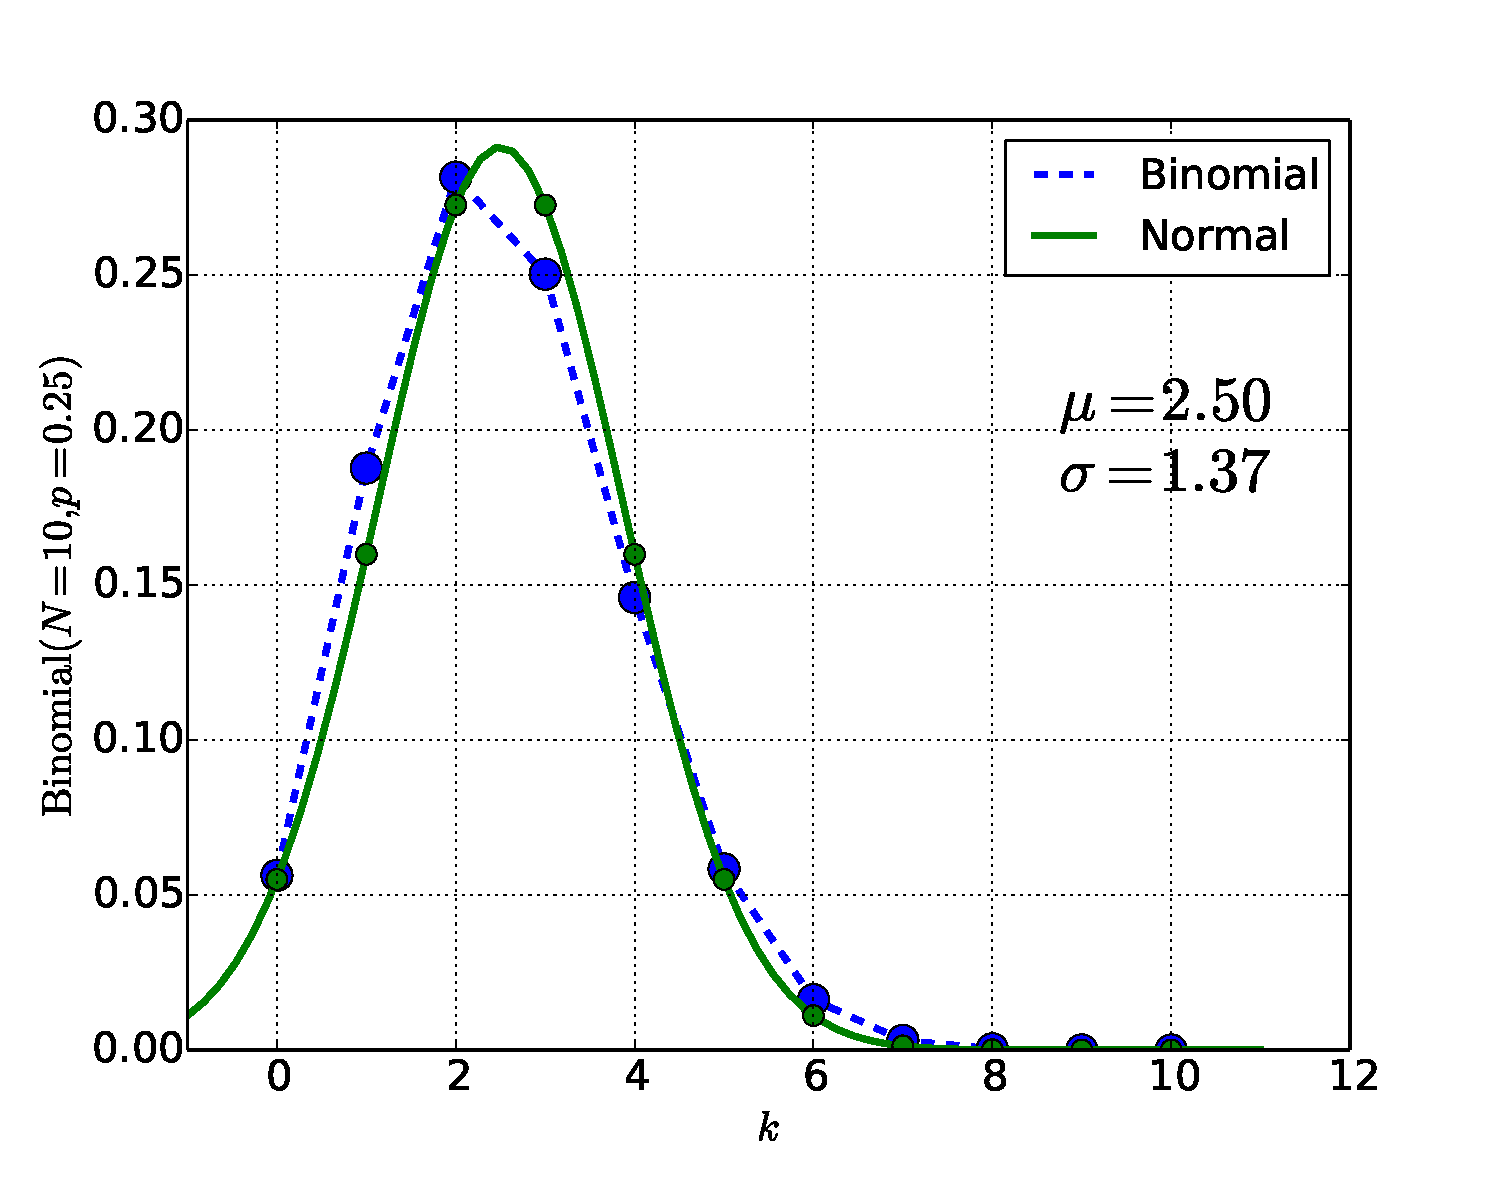
\includegraphics{binomial_normal1}

and

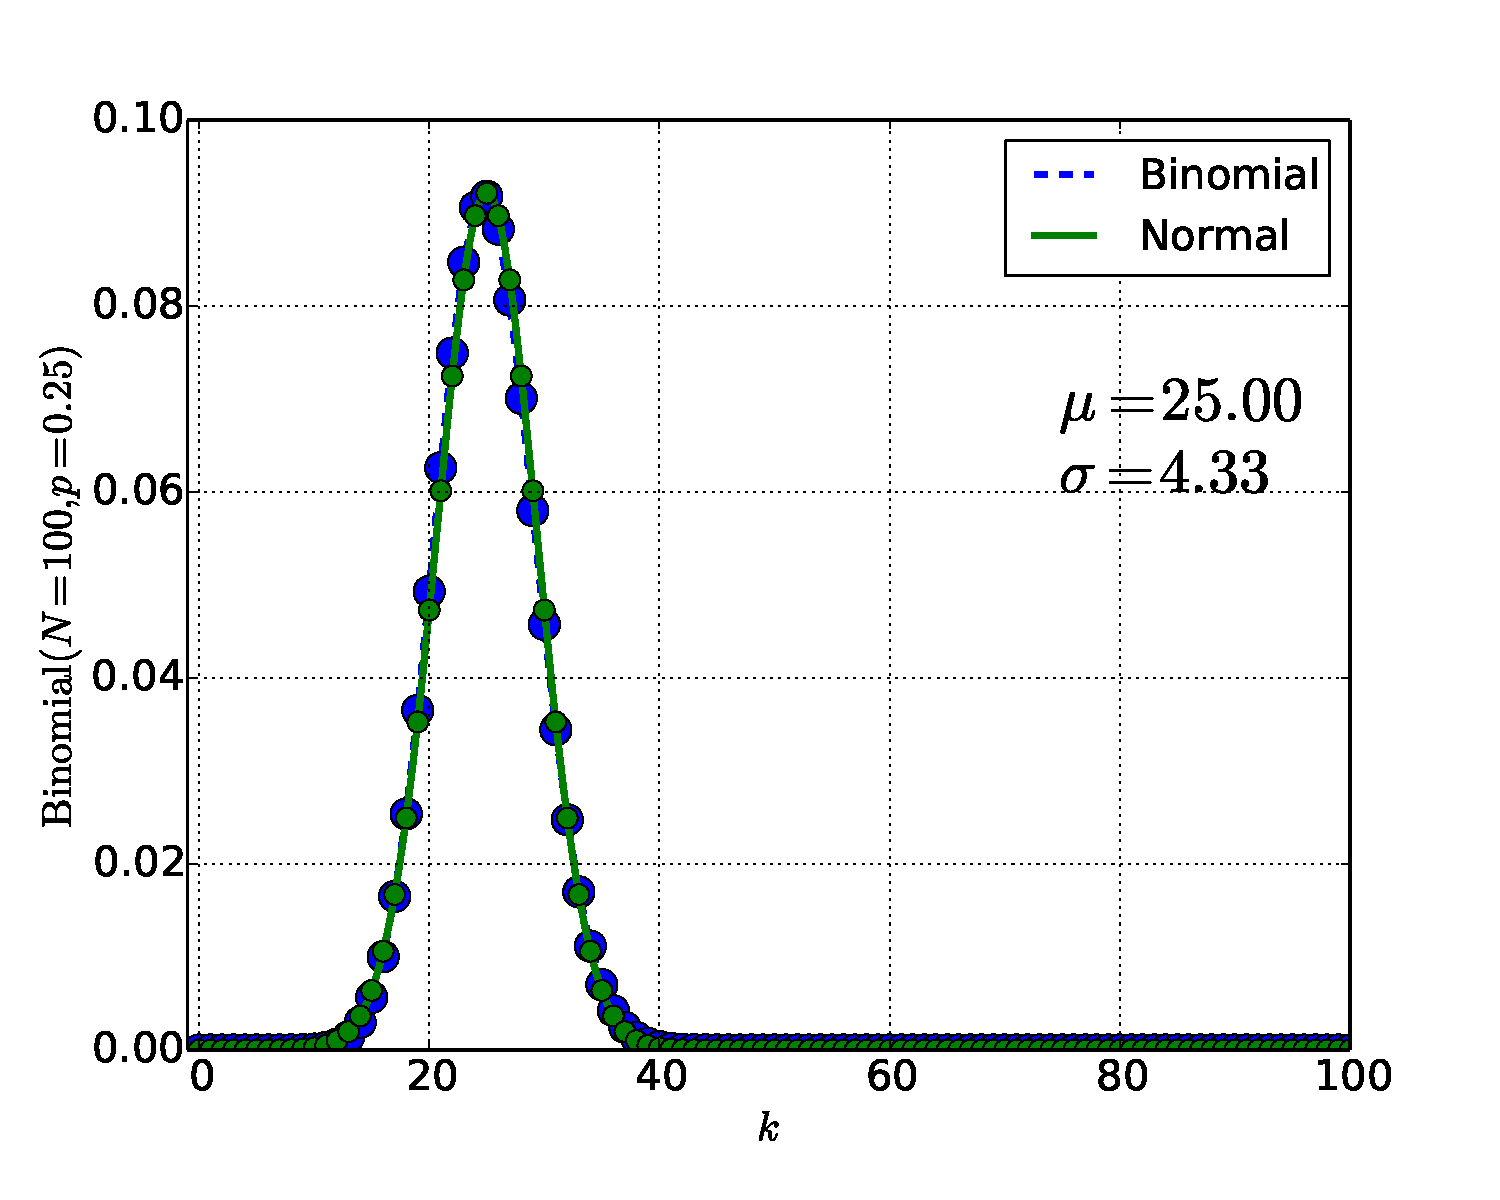
\includegraphics{binomial_normal2}

\subsection{The Student's $t$ Distribution}\label{sec:normal_t_approx}

For smallish data sets, $5<N<30$, we can replace the estimate of the mean from the Student's $t$ distribution to a Normal distribution with an increased estimate for the deviation.  It then becomes practical to use the more convenient $z$-score to estimate credible intervals rather than the full $t$ tables.  The approximation in this domain looks like\cite{berry1996statistics}

\highlight{Normal Approximation to the Student's {\em t} Distribution}{
For smallish data sets, $5<N<30$, 
\beqn
{\rm Student}_{{\rm dof}=N-1}(\bar{x}, S/\sqrt{N})&\sim& {\rm Normal}(\bar{x}, Sk/\sqrt{N}) \\
k&\equiv& 1+\frac{20}{N^{2}}
\eeqn
}{
For smallish data sets, $5<N<30$, 
\beqn
\lefteqn{{\rm Student}_{{\rm dof}=N-1}(\bar{x}, S/\sqrt{N})\sim}\\
&& {\rm Normal}(\bar{x}, k\cdot S/\sqrt{N})\\
k&\equiv& 1+\frac{20}{N^{2}}
\eeqn
}

\example{Estimating the True Length of an Object...Yet Again}
Say we have an object, and 5 measurements of its length from the same ruler but from different people,
\begin{center}
5.1\cm, 4.9\cm, 4.7\cm, 4.9\cm, 5.0\cm
\end{center}
Unlike earlier, let's say that we don't know the uncertainty (given this ruler) of one measurement.  What is the best estimate of the length?  Again, the best estimate should be given by the sample mean of these 5 samples,
\beqn
\hat{\mu} &=& \frac{x_{1} + x_{2} + \cdots + x_{N}}{N} \\
 &=& \frac{5.1\cm+ 4.9\cm+ 4.7\cm+ 4.9\cm+ 5.0\cm}{5} =4.92\cm
\eeqn
with uncertainty related to the adjusted sample deviation,
\beqn
S^{2}&=&\frac{1}{N-1}\left( (x_{1}-\bar{x})^{2}+\cdots+(x_{N}-\bar{x})^{2}\right) \\
&=&\frac{1}{5-1}\left( (5.1\cm-4.92\cm)^{2}+(4.9\cm-4.92\cm)^{2}+(4.7\cm-4.92\cm)^{2}+\right.\\
&&\left.(4.9\cm-4.92\cm)^{2}+(5.0\cm-4.92\cm)^{2}\right) \\
&=&0.024 \cm^{2}\\
S&=&\sqrt{0.024 \cm^{2}}=0.155\cm \\
\frac{S}{\sqrt{N}}&=&\frac{0.155\cm}{\sqrt{5}}=0.069\cm\\
k&=&1+\frac{20}{5^{2}}=1.8\\
k\cdot \frac{S}{\sqrt{N}}&=&1.8 \cdot 0.069\cm=0.124\cm
\eeqn
yielding a final best estimate of
\beqn
\hat{\mu} &=& 4.92\cm\pm 0.124\cm
\eeqn
or (with $2\sigma$ range),
\beqn
4.92\cm, 95\%\mbox{ CI} = [4.672\cm,5.168\cm]
\eeqn
Compare this range to the one shown in Example~\ref{ex:length_tdist} on page~\pageref{ex:length_tdist}.  The one here has a slightly larger range, which is a bit more conservative than is needed, but the calculation is quite a bit easier.

\section{Summary}

It is useful to see all of these results stemming from the same Bayes' Recipe, applied to different models of the data and (possibly) different prior probabilities.  As we have stated, many of the simple cases have been worked out by the mathematicians, so we don't need to do the work of deriving them.  It will be our task to understand their properties, to be able to apply them to real problems, and to understand their consequences.  One of the immediate observations that we make is the prevalence of the {\em Normal} distribution, justifying our detailed exploration of it in this chapter.

\newcommand{\postlikeprior}[3]{
	\beqn \underbrace{#1}_{\rm posterior\ probability} \sim \overbrace{#2}^{\rm likelihood}\times \underbrace{#3}_{\rm prior\ probability}
	\eeqn
}

\be
\i {\textbf{\textit{ Proportions}}}
	\bi
	\i[\bf Parameter of Interest:] $\theta$, the chances of a single event
	\i[\bf Applications:] coin flips, voting percentages, success in sports, performance on tests
	\i[\bf Form of the data:] $h$ successes in $N$ total events
	\i[\bf Model of the data:] 
	\beqn
	{\rm data} = \left\{\begin{array}{cl}
			{\rm success} & \mbox{, with probability $\theta$} \\
			{\rm failure} & \mbox{, otherwise (i.e. with probability $1-\theta$})
			\end{array}\right.
	\eeqn
	\i[\bf Posterior Probability:]
	\beqn \underbrace{{\rm Beta}(\theta|{\rm data})}_{\rm posterior\ probability} \sim \overbrace{ {\rm Binomial}({\rm data}|\theta)}^{\rm likelihood}\times \underbrace{{\rm Uniform}(\theta)}_{\rm prior\ probability}
	\eeqn
	\ei
\i {\textbf{\textit{Magnitude with Known Deviation}}}	\bi
	\i[\bf Parameter of Interest:] $\mu$, the true magnitude of a quantity, given the deviation, labeled by $\sigma$, from the central value
	\i[\bf Applications:] percentages with large samples, scientific measurements such as weight and size of objects, time scales of events
	\i[\bf Form of the data:] $N$ total data points, labeled $x_{1}, x_{2}, \cdots, x_{N}$, and given known $\sigma$
	\i[\bf Model of the data:] 
	\beqn
	{\rm data} = \mu + \mbox{uncertainty with probability Normal($\mu=0$,known $\sigma$)}
	\eeqn
	\i[\bf Posterior Probability:]
	\postlikeprior{{\rm Normal}(\mu_{2}|{\rm data},\sigma)}{{\rm Normal}({\rm data}|\mu,\sigma)}{{\rm Uniform}(\mu)}
	\ei
\i {\textbf{\textit{Magnitude with Unknown Deviation}}}	\bi
	\i[\bf Parameter of Interest:] $\mu$, the true magnitude of a quantity, and the unknown deviation, labeled by $\sigma$, from the central value
	\i[\bf Applications:] scientific measurements with small samples (less than around 30), such as weight and size of objects, time scales of a small number of events
	\i[\bf Form of the data:] $N$ total data points, labeled $x_{1}, x_{2}, \cdots, x_{N}$
	\i[\bf Model of the data:] 
	\beqn
	{\rm data} = \mu + \mbox{uncertainty with probability Normal($\mu=0,\sigma$)}
	\eeqn
	\i[\bf Posterior Probability:]
	\postlikeprior{{\rm P}(\mu,\sigma|{\rm data})}{{\rm Normal}({\rm data}|\mu,\sigma)}{{\rm Uniform}(\mu)\cdot{\rm Uniform}(\log \sigma)}
	\beqn 
	\underbrace{{\rm Student-T}(\mu|{\rm data})}_{\rm posterior\ probability} \sim \left[{\rm P}(\mu,\sigma|{\rm data})\right]_{\mbox{\scriptsize marginalized over $\sigma$}}
	\eeqn
	\beqn 
	\underbrace{{\rm F}(\sigma|{\rm data})}_{\rm posterior\ probability} \sim \left[{\rm P}(\mu,\sigma|{\rm data})\right]_{\mbox{\scriptsize marginalized over $\mu$}}
	\eeqn
	\ei
\ee





\section{Computer Examples}
\begin{fullwidth}
\begin{lstlisting}
from sie import *
\end{lstlisting}

\subsection{Estimating Lengths}


\subsubsection{Known deviation, $\sigma$}


\begin{lstlisting}
x=[5.1, 4.9, 4.7, 4.9, 5.0]
sigma=0.5
\end{lstlisting}

\begin{lstlisting}
mu=sample_mean(x)
N=len(x)
\end{lstlisting}

\begin{lstlisting}
dist=normal(mu,sigma/sqrt(N))
distplot(dist)
\end{lstlisting}

\begin{verbatim}
<matplotlib.figure.Figure at 0x10713c710>\end{verbatim}

\begin{center}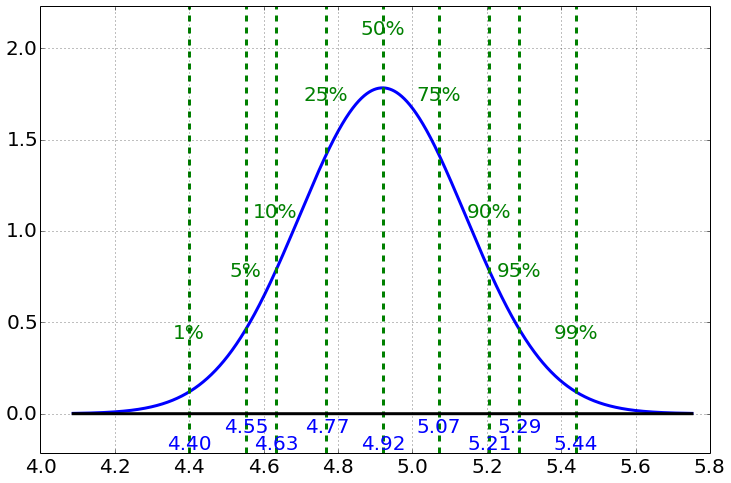
\includegraphics[width=4.5in]{Priors_Likelihoods_and_Posteriors/Priors_Likelihoods_and_Posteriors_fig0.png}\end{center}

\begin{lstlisting}
credible_interval(dist)
\end{lstlisting}

\begin{verbatim}
(4.4817387297117088, 4.9199999999999999, 5.358261270288291)
\end{verbatim}

\subsubsection{Unknown $\sigma$}


\begin{lstlisting}
mu=sample_mean(x)
s=sample_deviation(x)
print mu,s
\end{lstlisting}

\begin{verbatim}
4.92 0.148323969742
\end{verbatim}

\begin{lstlisting}
dist=tdist(N-1,mu,s/sqrt(N))
\end{lstlisting}

\begin{lstlisting}
distplot(dist,xlim=[4.6,5.4])
\end{lstlisting}

\begin{verbatim}
<matplotlib.figure.Figure at 0x1085b5c50>\end{verbatim}

\begin{center}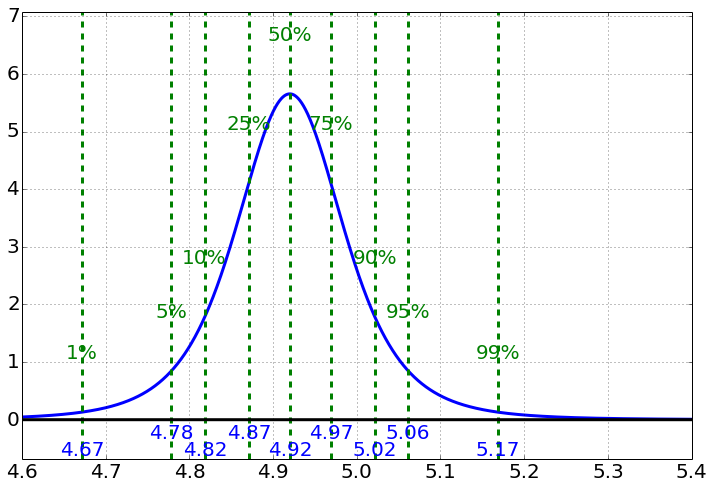
\includegraphics[width=4.5in]{Priors_Likelihoods_and_Posteriors/Priors_Likelihoods_and_Posteriors_fig1.png}\end{center}

\begin{lstlisting}
credible_interval(dist)
\end{lstlisting}

\begin{verbatim}
(4.7358314667008017, 4.9199999999999999, 5.1041685332991982)
\end{verbatim}

\begin{lstlisting}

\end{lstlisting}


\end{fullwidth}
